The \textit{DLR Institute for the Protection of Maritime Infrastructures} (DLR-MI) is consistently working on systems to improve the situational awareness of maritime infrastructures. Part of those awareness systems is the near real-time tracking of vessels and the detection of abnormal ship behavior. These anomalies can potentially range from unusual trajectories, entry into restricted zones, speeding and intentional AIS on-off switching to actual collisions or pirate attacks.
\par
This thesis focuses on the construction of a system and an associated robust model that is capable of predicting accurate future vessel trajectories. A component like this is a promising solution to discover irregular ship behavior. To this extent, the ability to generate end-to-end trajectories is an advantageous addition to any maritime surveillance system which can then be utilized in a variety of different tasks, especially the detection of abnormal vessel trajectories and collision avoidance.
However, building such a sophisticated model is a challenging task because real-world ship maneuvering not only depends on movement indicators (current position, speed, heading) but also on a wide range of non-kinematic factors (e.g., weather conditions, current, tides, and surrounding ships). Admittedly, only the kinematic factors are considered in this thesis due to time concerns. In addition to the potentially high-dimensional and semantically varying feature space, a suitable system has to also incorporate a time component and retain low computational costs, intending to potentially provide near real-time predictions in short time intervals.
\par
Previous work at the institute regarding this topic involved the usage of sequential models like LSTMs \cite[]{hochreiter1997long}. The downside of those network architectures is the requirement of a predefined frame of timestamps as input that eventually leads to a prediction of a fixed output window. An end-to-end path prediction has low performance due to the observed phenomena that sequentially taking a predicted output as input sequence leads to significant error accumulation.
\par
With the rise of deep reinforcement learning and its successful application in fields like robotics and autonomous system (\cite{s18092905, zare2021continuous, 9195789, martinsen2018curved}), the question comes to mind if the task of vessel path prediction can be formulated as a reinforcement learning problem as well. The idea behind using reinforcement learning is that training an agent to control an unmanned vessel results in a policy that learns end-to-end trajectories to get to a desired destination. While dropping the need for a dedicated simulation of the real-world, the abstract vessel trajectories are constructed solely based on historical AIS records. The agent is then forced to choose suitable values for the speed and heading of the ship. In combination with extensive tweaking of the state representation and reward function, the assumption is that the agent learns to mimic normal vessel behavior to eventually predict end-to-end trajectories.
\par
Using the word "mimic" in the previous paragraph reveals that this task is potentially better placed in the realm of \textit{Imitation Learning}, an approach that operates in the same mathematical framework as reinforcement learning and is very closely related to it. Besides an in-depth investigation of classical interactive reinforcement learning, we will also explore the performance when learning from expert demonstrations and trying to mimic human captain behavior.
\par
To give an example of what the agent should eventually learn, we illustrate two density maps of vessel trajectories generated by \cite{martinetraffic} for the year 2020:
\begin{figure}[H]
    \centering
    \begin{minipage}{.47\textwidth}
      \centering
      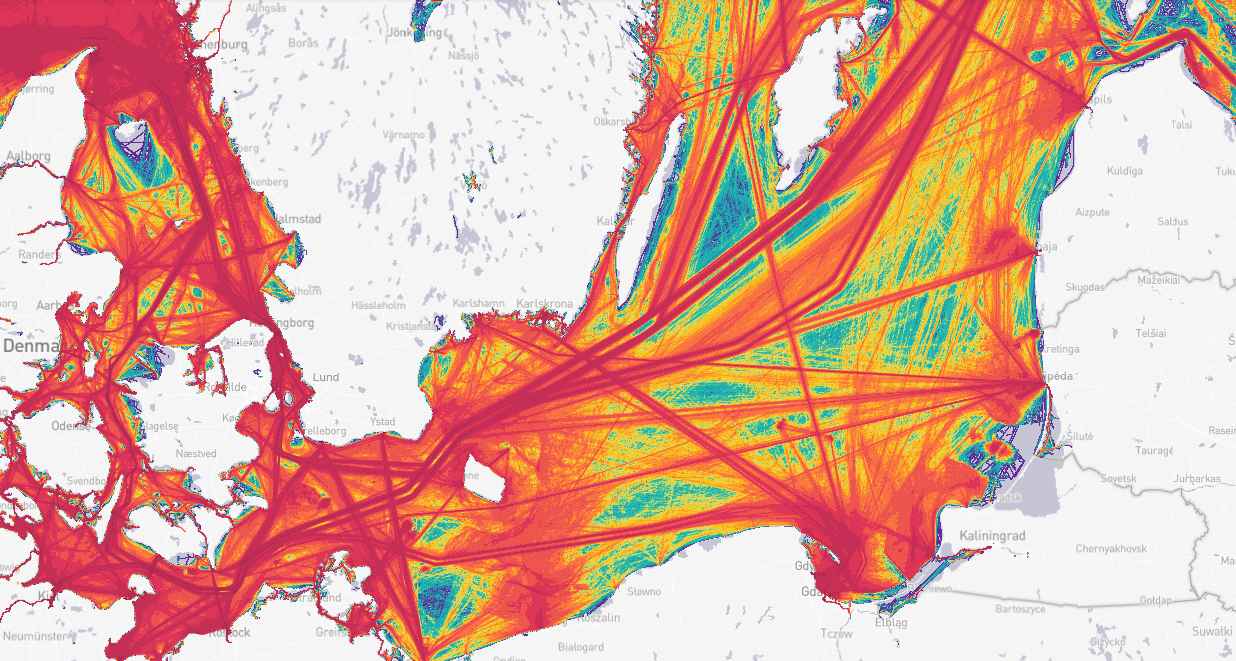
\includegraphics[width=\textwidth]{images/balticsea_density_routes.PNG}
      \captionof{figure}{Density map of vessel trajectories in the Baltic Sea.}
      \label{fig:baltic}
    \end{minipage}
    \hspace{.05\textwidth}%
    \begin{minipage}{.47\textwidth}
        \centering
        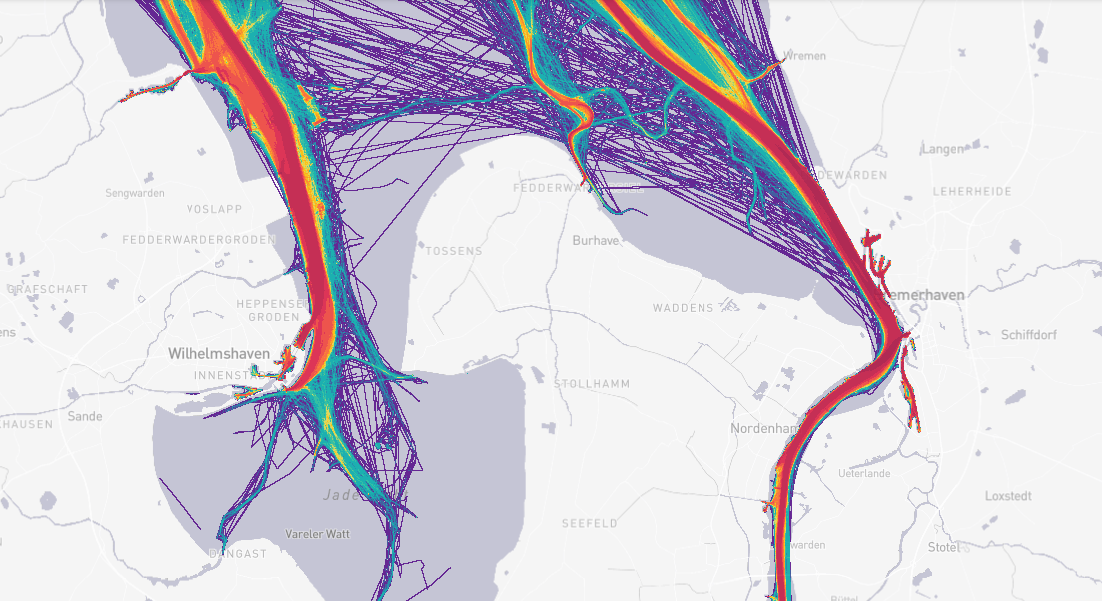
\includegraphics[width=\textwidth]{images/bhv_jadebusen_density_routes.PNG}
        \captionof{figure}{Density map of vessels near Bremerhaven and the Jadebusen.}
        \label{fig:jadebusen}
      \end{minipage}
\end{figure}
Looking at Fig. \ref{fig:baltic}, we can discover the international shipping routes by following the red lines which indicate a high volume of vessel traffic. Furthermore, we notice certain points where the majority of ships choose to suddenly change their heading. It is up to the agent to learn exactly those specific patterns as in break points, entry angles to the ports, speed values etc. In contrast to the big scope of international routes in Fig. \ref{fig:baltic}, a path prediction system can also be applied to a smaller more granular observation window as illustrated in Fig. \ref{fig:jadebusen}. By "granular" we mean the focus on rapid decision sequences in short time intervals when entering and maneuvering in or near a port. As the author's university and the DLR-MI is located in Bremerhaven, the observation window and scope is centered around the city's port. Fortunately, the harbor of Bremerhaven is also one of the largest ports in Europe with more than 4.7 million TEUs (twenty-foot equivalent unit) in sea goods and a massive car terminal with an automobile throughput of 1,733,100 cars being handled in the year 2020  \cite[]{bremenports}.